
\begin{figure}[H]
  {
    \setlength{\tabcolsep}{3.0pt}
    \setlength\cmidrulewidth{\heavyrulewidth} % Make cmidrule = 
    \begin{adjustbox}{width=3cm,center}
      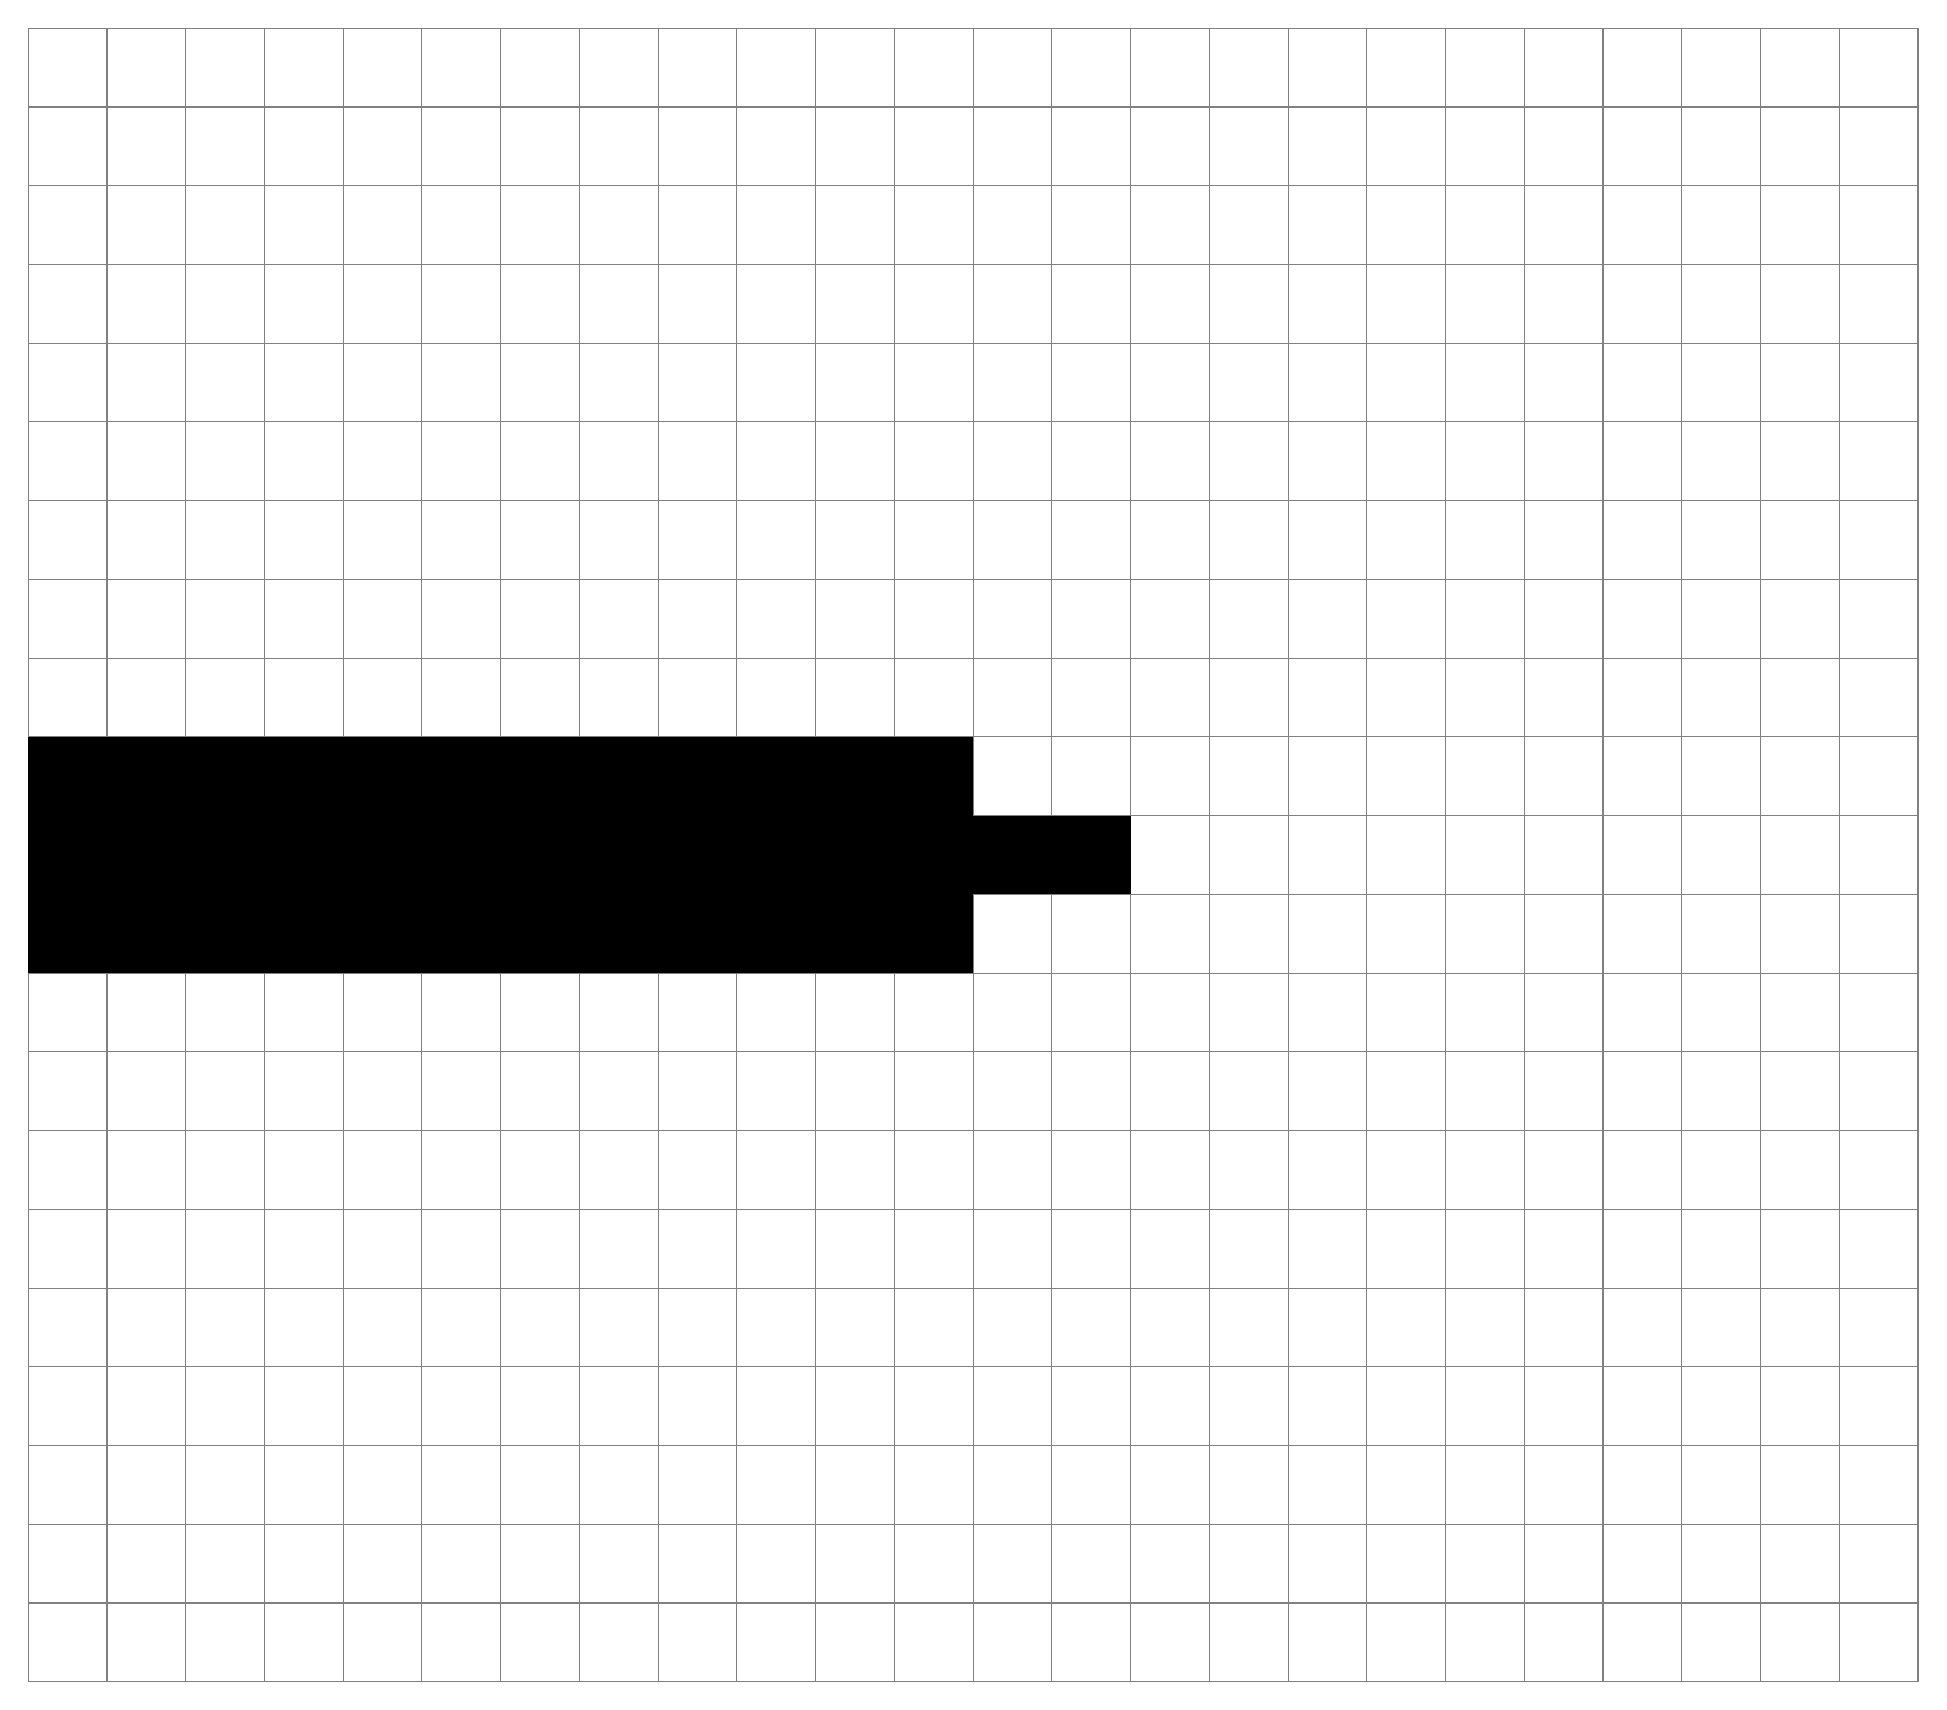
\begin{tikzpicture}

	\draw[step=1.0,gray,thin] (0,0) grid (24,21);
	\fill[\SPRITECOLOR] (0,11) rectangle ++ (1,1);
	\fill[\SPRITECOLOR] (1,11) rectangle ++ (1,1);
	\fill[\SPRITECOLOR] (2,11) rectangle ++ (1,1);
	\fill[\SPRITECOLOR] (3,11) rectangle ++ (1,1);
	\fill[\SPRITECOLOR] (4,11) rectangle ++ (1,1);
	\fill[\SPRITECOLOR] (5,11) rectangle ++ (1,1);
	\fill[\MULTICOLORTWO] (6,11) rectangle ++ (1,1);
	\fill[\MULTICOLORTWO] (7,11) rectangle ++ (1,1);
	\fill[\MULTICOLORONE] (8,11) rectangle ++ (1,1);
	\fill[\MULTICOLORONE] (9,11) rectangle ++ (1,1);
	\fill[\MULTICOLORONE] (10,11) rectangle ++ (1,1);
	\fill[\MULTICOLORONE] (11,11) rectangle ++ (1,1);
	\fill[\SPRITECOLOR] (0,10) rectangle ++ (1,1);
	\fill[\SPRITECOLOR] (1,10) rectangle ++ (1,1);
	\fill[\SPRITECOLOR] (2,10) rectangle ++ (1,1);
	\fill[\SPRITECOLOR] (3,10) rectangle ++ (1,1);
	\fill[\SPRITECOLOR] (4,10) rectangle ++ (1,1);
	\fill[\SPRITECOLOR] (5,10) rectangle ++ (1,1);
	\fill[\MULTICOLORTWO] (6,10) rectangle ++ (1,1);
	\fill[\MULTICOLORTWO] (7,10) rectangle ++ (1,1);
	\fill[\MULTICOLORONE] (8,10) rectangle ++ (1,1);
	\fill[\MULTICOLORONE] (9,10) rectangle ++ (1,1);
	\fill[\MULTICOLORONE] (10,10) rectangle ++ (1,1);
	\fill[\MULTICOLORONE] (11,10) rectangle ++ (1,1);
	\fill[\MULTICOLORONE] (12,10) rectangle ++ (1,1);
	\fill[\MULTICOLORONE] (13,10) rectangle ++ (1,1);
	\fill[\SPRITECOLOR] (0,9) rectangle ++ (1,1);
	\fill[\SPRITECOLOR] (1,9) rectangle ++ (1,1);
	\fill[\SPRITECOLOR] (2,9) rectangle ++ (1,1);
	\fill[\SPRITECOLOR] (3,9) rectangle ++ (1,1);
	\fill[\SPRITECOLOR] (4,9) rectangle ++ (1,1);
	\fill[\SPRITECOLOR] (5,9) rectangle ++ (1,1);
	\fill[\MULTICOLORTWO] (6,9) rectangle ++ (1,1);
	\fill[\MULTICOLORTWO] (7,9) rectangle ++ (1,1);
	\fill[\MULTICOLORONE] (8,9) rectangle ++ (1,1);
	\fill[\MULTICOLORONE] (9,9) rectangle ++ (1,1);
	\fill[\MULTICOLORONE] (10,9) rectangle ++ (1,1);
	\fill[\MULTICOLORONE] (11,9) rectangle ++ (1,1);

      \end{tikzpicture}
    \end{adjustbox}
  }\caption{FLYING\_BAR2}
\end{figure}
